\chapter{Related Works}
\label{ch:related_works}
In this chapter we review the main challenges in the application of reinforcement learning in the
field of robotics and what are the state of the art algorithms and techniques. 
Next, hierarchical reinforcement learning is introduced and a brief overview of the different frameworks is presented.

\section{Robotics}
Traditional methods in robotics require expert knowledge and very accurate models of the controlled robot in order to achieve a given task.
Usually, the desired behavior of the robot is specified using some planned trajectories with a given structure, e.g. cubic splines, that are then optimized
using some criterion. For example, the objective function could include the path smoothness, distance to obstacles, time, path lengths and the robot constraints.

An example of these techniques is given by \cite{baseline}, where the authors implemented an algorithm for the Air Hockey hit task described in \ref{subsec:qualifying_stage} using a general purpose robot with 7 DoFs.
The end-effector's trajectory for hitting the puck is planned avoiding collisions and then optimized with multiple optimization problems in order to achieve high
performance while adhering to the constraints :

\textbf{Weighted Null Space Optimization}:
To achieve high speed trajectories, the null space velocity is optimized at every point of the trajectory. Considering only the position of the end-effector in task space,
the concerned Jacobian is $J_p \in \mathbb{R}^{3\times n}$, where $n$ is the number of joints. Let $b = J^\dag_p\left(\frac{\bar{x} - x}{\Delta T} + \bar{v}\right)$
be the joint velocities for the trajectory tracking with $J_p^\dag = J^\intercal\left(J J^\intercal\right)^{-1}$ being the general pseudoinverse of $J_p$, $x$, $\bar{x}$, $\bar{v}$ are respectively actual, desired cartesian position and desired cartesian velocity.
The objective is to maximize the weighted joint velocity as

\begin{equation*}
    \begin{aligned}
        \min_\alpha  \quad&\frac{1}{2} \Vert b + E_N \alpha \Vert^{2}_W \\
        \text{s.t.}  \quad&\dot{q}^{\min} \le b + E_N \alpha \le \dot{q}^{\max}
    \end{aligned}
\end{equation*}

where $E_N \in \mathbb{R}^{n\times \left(n - 3\right)}$ is the \textit{null space matrix}. Each column of the \textit{null space matrix} is one basis vector of
$Null(J_p)$ and $\alpha \in \mathbb{R}^{n-3}$ are entries on each basis vector. It should be pointed out that, when $W$ is set to be an identity matrix, the optimal solution
is $\alpha = 0$ when the constraints are not violated. In practice higher weights are applied on joints that afford more loads and have lower velocity limits.
The next step and velocity are obtained by Euler integration

\begin{equation*}
    \begin{aligned}
        &\dot{q}_{next} = b + E_N \alpha^* \\
        &q_{next} = q_{current} + \dot{q}_{next} \Delta T
    \end{aligned}
\end{equation*}

\textbf{Hitting Configuration Optimization}:
To find the best configuration for the hitting movement, the manipulability along a specific hitting direction $v$ is considered, as presented in \cite{manipulability}.
The following quantity at the hitting point $p$ is maximized

\begin{equation*}
    \begin{aligned}
        \max_q \quad& \Vert \left(v^\intercal J_p(q) \right) \Vert_2, \\
        \text{s.t.} \quad& FK_p(q) = p
    \end{aligned}
\end{equation*}

where $FK_p(q)$ is the forward kinematic w.r.t the end-effector position.


\textbf{Computing the maximum hitting velocity}:
To compute the maximum hitting velocity at the selected hitting configuration, two strategies can be used:
\begin{enumerate}
    \item \textit{Least Square solution}: The hitting speed velocity is parameterized as a scalar $\eta$ and a hitting direction $v$, such that
        $v_{\max} = \eta v$. The least square solution is $\dot{q} = J_p^\dag(q^*)v_{\max}$. Thus, the maximum possible joint velocity can be determined
        by the minimum ratio of the absolute value of the \textit{i}-th joint velocity $\dot{q}_i$ and its maximum $\dot{q}^{\max}_i$

        \begin{equation*}
            \eta = \min_i \left(\frac{\dot{q}^{\max}_i}{|\dot{q}_i|}\right),\quad i \in \{1,\dots,n\}.
        \end{equation*}

    \item \textit{Linear Programming}:  Instead of using the least squared solution, a linear program on the null space can be constructed as

        \begin{equation*}
            \begin{aligned}
                \max_\alpha \quad &v^\intercal J_p(q^*)\left(E_{v^\bot}(q^*)\alpha\right), \\
                \text{s.t.} \quad & \dot{q}^{\min} \le E_{v^\bot}(q^*)\alpha \le \dot{q}^{\max},
            \end{aligned}
        \end{equation*}

        where $v^\bot \in \mathbb{R}^3$ is the orthogonal complement space of $v \in \mathbb{R}^3$, which in this case is a plane orthogonal to the hitting direction,
        and $E_{v^\bot}(q^*) = Null\left[(v^{\bot})^\intercal J_p(q^*)\right]$ is the basis vectors spanning the null space of $(v^{\bot})^\intercal J_p(q^*)$.
\end{enumerate}


\section{Reinforcement Learning in Robotics}
Reinforcement Learning enables robots to learn complex behaviors through interaction with the environment and maximizing the cumulative rewards.
This can be particularly advantageous for tasks that are too intricate or dynamic to be effectively addressed by conventional methods.
On the other hand traditional robotics techniques, such as classical control theory and model-based approaches, are typically more predictable and easier to implement.
While these techniques may lack the flexibility and adaptability of reinforcement learning, they offer a more straightforward and less resource-intensive path to deploying
functional robotic systems. Reinforcement Learning in Robotics has however many challenges to face \cite{Kober2013}, and these are described in the following section.

\subsubsection{Curse of Dimensionality}
Robotics systems often have to deal with high dimensional state and action spaces due to the many degrees of freedom (DoFs) of modern
anthropomorfic robots. For example, in the ball-paddling task shown in Figure \ref{fig:ball_paddling_robot}, where a robotic arm need to maintain the ball bouncing on a racket, a proper representation
of s robot's state would consist of its joint angles and velocities for each of its seven DoFs as well as the cartesian position
and velocity of the ball. The robot's actions would be the generated motor commands, which often are torques or accelerations.
%In this example, we have $2\times\left(7 + 3\right)=20$ state dimensions and 7-dimensional continuous actions.

This curse of dimensionality presents significant challenges in terms of computational complexity 
and the effectiveness of learning algorithms.

\begin{figure}[H]
    \centering
    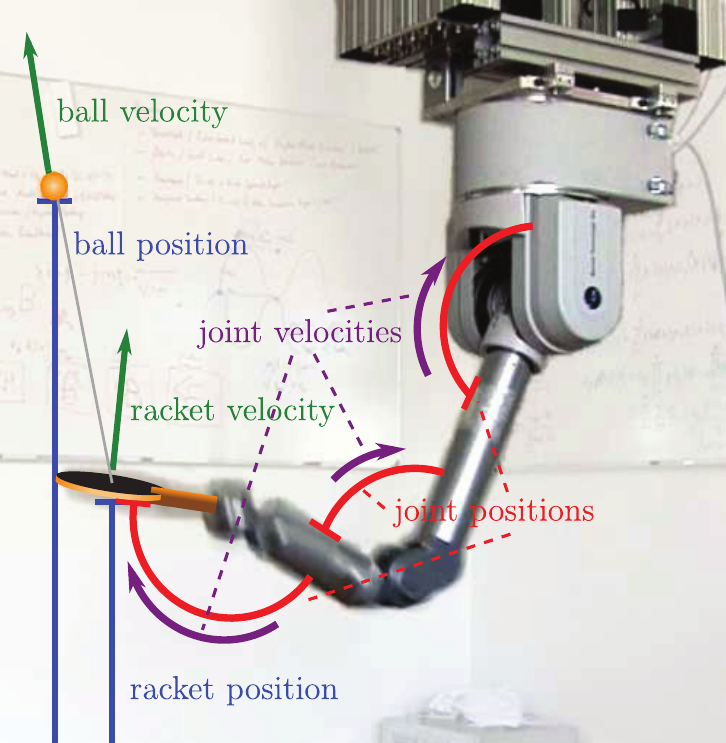
\includegraphics[width=0.3\textwidth]{Images/ball_paddling.png}
    \caption{Ball Paddling Robot}
    \label{fig:ball_paddling_robot}
\end{figure}

This problem is solved with function approximators like neural networks using Deep Reinforcement Learning algorithms.

\subsubsection{Curse of real-world samples}
%usura robot
Robots interact with the physical world, hence robot reinforcement learning suffers from most of the resulting real-world problems.
For example, robot hardware is usually expensive, suffers from wear and tear, and requires careful maintenance. This is why safe exploration
becomes a key issue in the learning process.

Several more aspects of the real-world make robotics a challenging domain. Frequently, the environment settings during an earlier 
learning period cannot be reproduced. This problem makes comparing algorithms particularly hard. Furthermore, the approaches often have to deal 
with uncertainty due to inherent measurement noise and the inability to observe all states directly with sensors.

%human supervision
Most real robot learning tasks require some form of human supervision, e.g. putting the pole back on the robot's end-effector during pole balancing
 after a failure. Even when an automatic reset exists, the learning speed becomes essential as a task on a real robot cannot be sped up.
In some tasks such as a slowly rolling robot, the dynamics can be ignored; in others such as a flying robot, they cannot. In particular in the latter case,
often the whole episode needs to be completed as it is not possible to start from arbitrary states.

For such reasons, real-world samples are expensive in terms of time, labor and, potentially, finances. In robotic reinforcement learning,
it is often considered to be more important to limit the real-world interaction time instead of limiting memory consumption or computational complexity.
Thus, sample efficient algorithms that are able to learn from a small number of trials are essential.

Since the robot is a physical system, there are strict constraints on the interaction between the learning algorithm
and the robot setup. For dynamic tasks, the movement cannot be paused and actions must be selected within a time-budget without 
the opportunity to pause to think, learn or plan between actions.

%discretization and delays
As reinforcement learning algorithms are inherently implemented on a digital computer, the discretization of
time is unavoidable despite the inherently continuous time configuration of physical systems. Time-discretization of the
actuation can generate undesirable artifacts. As most robots are controlled at fixed sampling frequencies (in the range between
500 Hz and 3 kHz) determined by the manufacturer of the robot, the upper bound on the rate of temporal discretization
is usually pre-determined. The lower bound depends on the horizon of the problem, the achievable speed of changes in
the state, as well as delays in sensing and actuation. All physical systems exhibit such delays in sensing and
actuation. The state of the setup (represented by the filtered sensor signals) may frequently lag behind the real state due
to processing and communication delays. More critically, there are also communication delays in actuation as well
as delays due to the fact that neither motors, gear boxes nor the body's movement can change instantly. Owing to
these delays, actions may not have instantaneous effects but are observable only several time steps later. In contrast, 
in most general reinforcement learning algorithms, the actions are assumed to take effect instantaneously as such
delays would violate the usual Markov assumption. This effect can be addressed by putting some number of recent
actions into the state. However, this significantly increases the dimensionality of the problem.
The problems related to time budgets and delays can also be avoided by increasing the duration of the time steps.
One downside of this approach is that the robot cannot be controlled as precisely.% another issue is that it may complicate a
%description of system dynamics.

%simulation
\subsubsection{Curse of under-modeling and model uncertainty}
One way to offset the cost of real-world interaction is to use accurate models as simulators. In an ideal setting, this
approach would make it possible to learn the optimal policy within the emulated environment and subsequently transfer it to the real robot.
Unfortunately, creating a sufficiently accurate model of the robot and its environment is challenging and often requires
very many data samples. As small model errors due to this under-modeling accumulate, the simulated robot can
quickly diverge from the real-world system.

Fot tasks where the system is self-stabilizing (that is, where the robot does not require active control to remain in a safe state or return to it),
transferring policies often works well. Nevertheless, tasks can often be learned better in the real world than in emulated environments due to complex mechanical interactions
that have proven difficult to model accurately. In contrast, in unstable tasks small variations have drastic consequences. %For example, in a pole balancing
%task, the equilibrium of the upright pole is very brittle and constant control is required to stabilize the system. Transferred policies often perform poorly
%in this setting.

\subsubsection{Curse of goal specification}
In reinforcement learning, the desired behavior is implicitly specified by the reward function. The goal of reinforcement
learning algorithms then is to maximize the accumulated long-term reward. %While often dramatically simpler than specifying the behavior itself
In practice, it can be surprisingly difficult to define a good reward function in robot reinforcement learning. 
%The learner must observe variance in the reward signal in order to be able to improve a
%policy: if the same return is always received, there is no way to determine which policy is better or closer to the optimum. 
In many domains, it seems natural to provide rewards only upon task achievement, for example, when a table tennis
robot wins a match. This view results in an apparently simple, binary reward specification. However, a robot may
receive such a reward so rarely that it is unlikely to ever succeed in the lifetime of a real-world system. Instead of
relying on simpler binary rewards, we frequently need to include intermediate rewards in the scalar reward function
to guide the learning process to a reasonable solution, a process known as \textit{reward shaping} \cite{Laud2004}.
This approach can add additional guidance to the agent, helping it learn the desired behavior faster by indicating that certain actions are beneficial.
However \textit{reward shaping} requires expert knowledge to ensure the rewards accurately reflect progress towards the goal.

% \subsubsection{SAC in Robotics}
% SAC \cite{SAC} achieves state of the art performance for robotic tasks in simulation and real-world scenarios as it is able to
% handle continuous state-action spaces and is an off-policy algorithm.
% As described in \cite{SAC_modified}, the authors successfully used SAC to learn policies for a quadrupedal locomotion task and
% a dexterous hand manipulation task in real-world. Being an off-policy algorithm SAC is more sample efficient than other on-policy
% algorithms like PPO \cite{PPO} and this helps mitigating the curse of real-world samples.

\section{ATACOM}
\label{sec:atacom}
One important factor that cannot be neglected in real-world applications is the necessity of satisfying constraints.
Many practical considerations can be formulated in the form of constraints, such as safety and mechanical viability. For example,
in the robot manipulation task, the robot should not take actions that damage the environment and cannot take actions that exceed
its feasible range of motion.

In order to achieve safe exploration during learning process in continuous control problems different algorithms have been developed.
This section describes the one that was employed in this thesis, ATACOM \cite{Atacom}
 
ATACOM transforms a constrained RL problem into a typical unconstrained RL problem. Hence the problem can be addressed by any
model-free RL algorithm while maintaining the constraints below the tolerance. Furthermore, ATACOM can handle both equality and inequality
constraints.

The state variable $s \in \mc{S}$ is decomposed in the directly controllable state $q \in \mc{Q}$ and uncontrollable state, i.e., $s = \left[\begin{smallmatrix} \bm{q} & \bm{x}\end{smallmatrix}\right]^\intercal$.
We assume that the constraints $\bm{c}(\bm{q}) \le \bm{0}$ are known and depend purely on the controllable state. 

The idea behind ATACOM is to construct the constraint manifold $\bm{\mc{M}_c} : \bm{c}(\bm{q}) = \bm{0}$, determine the bases $\bm{N_c}$ of the tangent space $\bm{\mc{T}_c}$
and sample state velocity in the tangent space (Figure \ref{fig:constraint_manifold}).

\begin{figure}[H]
    \centering
    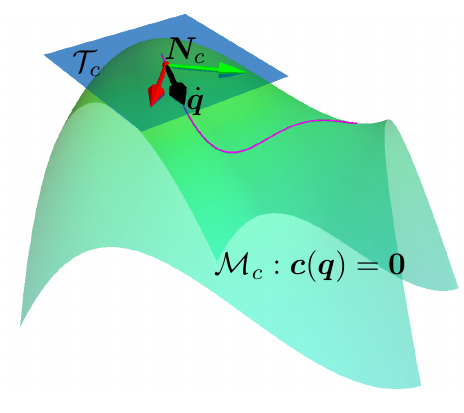
\includegraphics[width=0.3\textwidth]{Images/constraint_manifold.png}
    \caption[ATACOM]{
        Acting on the Tangent Space of the Constraint Manifold. The constraint set $\bm{c}(\bm{q}) = \bm{0}$ is a differentiable manifold
        $\mc{M}_c$ embedded in the original state space. A set of basis $\bm{N}_c$ is used to represent the span of tangent space $\bm{\mc{T}}_c$.
        The tangent space velocity/acceleration can be determined by a coordinate based on the basis, and the control action is determined based on the tangent
        space velocity/acceleration, the resulting trajectory is maintained on the constraint manifold.
        }
    \label{fig:constraint_manifold}
\end{figure}

% The state constraints are defined as
% \begin{equation}
%     \label{eq:state_constraints}
%     \bm{f}(\bm{q}) = \bm{0},\quad \bm{g}(\bm{q}) \le \bm{0},
% \end{equation}
% where $\bm{f} : \mathbb{R}^Q \to \mathbb{R}^F, \bm{g} : \mathbb{R}^Q \to \mathbb{R}^G$ are two $C^2$ mappings for $F$ equality and $G$ inequality
% constraints, and $F < q$. We add the slack variable $\bm{\mu} \in \mathbb{R}^G$ in inequality constraints to convert the original constraints \eqref{eq:state_constraints}
% into equality constraints

% \begin{equation}
%     \label{eq:state_constraints_2}
%     \bm{c(q,\mu)} =
%     \begin{bmatrix}
%         \bm{f}(\bm{q}) & \bm{g}(\bm{q}) + \frac{1}{2}\bm{\mu}^2
%     \end{bmatrix} = \bm{0}.
% \end{equation}

% The constaints set \eqref{eq:state_constraints_2} is a $(F + G)$ dimensional manifold embedded in $(Q + G)$ dimensional space. We calculate the time derivative
% of \eqref{eq:state_constraints_2}

% \begin{equation}
%     \bm{\dot{c}}(\bm{q},\bm{\mu},\bm{\dot{q}},\bm{\dot{\mu}}) = 
%     \begin{bmatrix}
%         \bm{J_f}(\bm{q}) & \bm{0} \\
%         \bm{J_g}(\bm{q}) & diag(\bm{\mu})
%     \end{bmatrix}
%     \begin{bmatrix}
%         \bm{\dot{q}} \\
%         \bm{\dot{\mu}}
%     \end{bmatrix}
%     = \bm{J_c}(\bm{q},\bm{\mu})
%     \begin{bmatrix}
%         \bm{\dot{q}} \\
%         \bm{\dot{\mu}}
%     \end{bmatrix},
% \end{equation}

% with the jacobians $\bm{J_f} \in \mathbb{R}^{F \times Q}$ and $\bm{J_g} \in \mathbb{R}^{G \times Q}$ of $\bm{f}(\bm{q})$ and $\bm{g}(\bm{q})$, respectively.
% Both Jacobians are combined into the Jacobian Matrix $\bm{J_c}(\bm{q}, \bm{\mu}) \in \mathbb{R}^{(F+G) \times (Q + G)}$ of the complete constraint set.

% We can find the null space matrix $\bm{N_c}(\bm{q}, \bm{\mu}) = Null\left[\bm{J_c}(\bm{q},\bm{\mu})\right] \in \mathbb{R}^{(Q+G)\times(Q-F)}$ via SVD.


The advantages of ATACOM can be summarized as follows:
\begin{itemize}
    \item It can deal both with \textbf{equality and inequality constraints}. All of the constraints at each time step are maintained
    below the tolerance during the whole process.
    \item It does not require an initial feasible policy, the agent can \textbf{learn from scratch}.
    \item It requires \textbf{no manual safe backup policy} to move the system back into the safe region.
    \item It can be applied to any model-free RL algorithm, using both \textbf{deterministic and stochastic policies}
    \item It can focus the exploration on the \textbf{lower-dimensional manifold} instead of exploring in the original action space
    for equality constrained problem.
    \item It has \textbf{better learning performance} as the inequality constraints restrict to a smaller feasible state-action space.
\end {itemize}

As a downside this method requires
\begin{itemize}
    \item differentiable constraint functions.
    \item a sufficiently accurate invertible dynamics model of the robot or a well-performed tracking controller.
\end{itemize}

% \begin{definition}
%     A Constrained Markov Decision Process (CMDP) is a tuple $(\mc{S}, \mc{A}, P, R, \gamma, \mc{C})$, where $\mc{S}$ is a state-space,
%     $\mc{A}$ is an action space, $P: \mc{S}\times\mc{A}\times\mc{S} \to [0,1]$ is a transition kernel, $\gamma$ is a discount factor,
%     and $\mc{C}: \left{c_i : \mc{S} \to \mathbb{R} | i \in 1, \dots, k}$ is a set of \textit{immediate state-constraint} functions.
% \end{definition}


\section{Hierarchical Reinforcement Learning}
When tasks are too complex, it is often easier to decompose it into more manageable sub-tasks. Hierarchical Reinforcement Learning
is a learning paradigm that aims to achieve this using temporal abstraction:

Reasoning on multiple time scales using temporally extended actions (sub-behaviors) that consist of a sequence of primitive actions
and possibly other temporally extended actions.

The following information is derived from \cite{survey_mdpi}.

\subsection{Options Framework}
Here, a popular framework to achieve temporal abstraction in reinforcement learning, the \textit{option framework} \cite{Options}, is described.

\begin{definition}
    An Option is a tuple $\omega = (I, \pi, \beta)$ where
    \begin{itemize}
        \item $I \in \mc{S}$ is the initiation set, which defines the states in which the option can be initiated
        \item $\beta: \mc{S} \rightarrow [0, 1]$ is the termination condition that decides when an option will halt its execution
        \item $\pi: \mc{S} \times \mc{A} \rightarrow [0,1]$ is the intra-option policy.
    \end{itemize}
\end{definition}

A policy-over-options $\pi(\omega|s_t)$ selects an option $\omega \in \Omega$ given a state $s_t$. This additional policy can be useful
to select the best options, when the current state belongs to multiple option initiation sets. It can also be used as an alternative to defining
an initiation set for each option.

The most often used execution model is the call-and-return model. This approach is often also called hierarchical-execution.
In this model a policy-over-options selects an option according to the current state. The agent follows this option until the 
agent triggers the termination condition of the active option.

\begin{figure}[b]
    \centering
    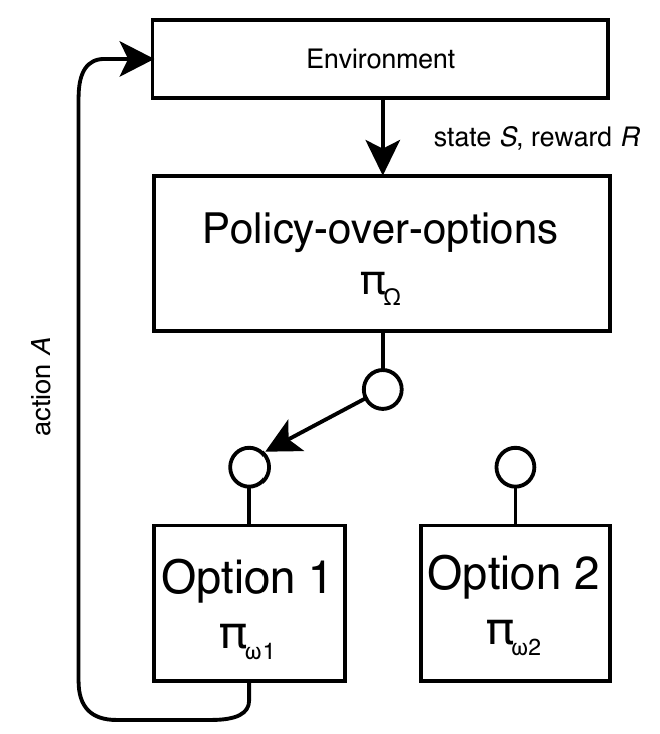
\includegraphics[width=0.3\textwidth]{Images/options_framework.png}
    \caption{Options framework}
    \label{fig:options_framework}
\end{figure}

Motion templates \cite{motion_templates} are options that can be parameterized in order to adapt the behavior of its intra-option policy.
This is often useful in a continuous state-space. A motion template could for example be discovered for throwing a ball. The exhibited
force and angle might be parameters of this template. Learning a single policy for each possible combination of force-angle would be infeasible.

\subsubsection{Option-Critic Framework}

The task of learning options can be decoupled from learning the policy-over-options. The agent can focus first on finding useful temporal
abstractions that simplify the environment. However, this approach of bottom-up learning risks wasting time on learning sub-behaviors which might not be required
in order to solve the problem at hand. Formulating options development and discovery as part of an optimization problem aimed at maximizing the
total future reward is an alternative approach, which allows options and a policy-over-options to be learned end-to-end.

The Option-Critic architecture (OC) \cite{option-critic} is an end-to-end framework capable of discovering and developing options without
using prior knowledge. The actor part in the OC framework consists of multiple intra-options policies. The critic part is capable of assessing discounted
future value of options and actions.

PPOC \cite{PPOC} extends the Option-Critic algorithm for continuous control tasks using PPO \cite{PPO}, a popular on-policy deep reinforcement learning algorithm.

\begin{figure}[H]
    \centering
    \label{fig:options_critic}
    \caption{Option-Critic Architecture.}
    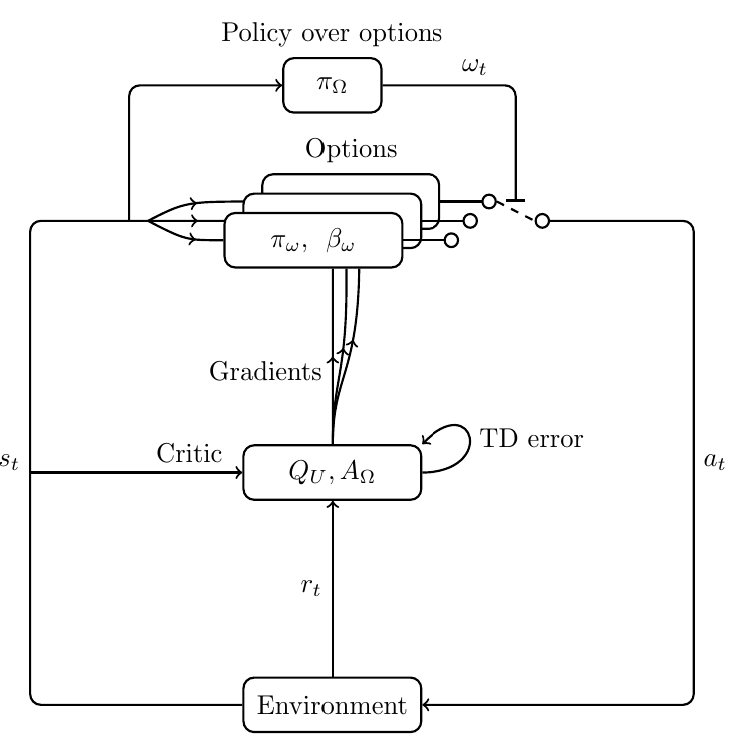
\includegraphics[scale=0.2]{Images/option-critic.png}
\end{figure}

\subsection{Goal-Conditional Framework}

Options are difficult to scale to support numerous sub-behaviors. Training options is inefficient because usually only
one option is trained at the time and no components are shared between them.

Here a different approach is presented; the goal-conditional framework.

The goal-conditional framework models sub-behaviors differently. In order to support a large amount of sub-behaviors,
a goal-vector $z \in Z$ is utilized to express different sub-behaviors.
The goal-vector characterizes the desired sub-behavior activated by a higher level manager to a lower level worker.
The idea is illustrated in Figure \ref{fig:goal-conditional}. This goal-vector can be discrete in order to express
a limited number of abstractions, but it is also possible to use a continuous vector to express an infinite number of possible abstractions.


\begin{figure}
    \centering
    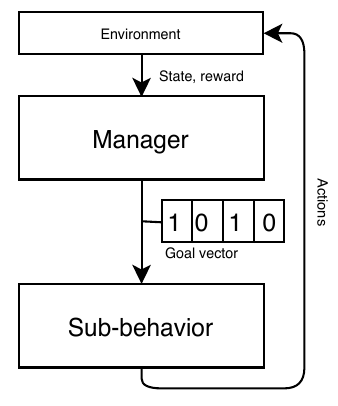
\includegraphics[width=0.3\textwidth]{Images/goal-conditional.png}
    \caption{Goal-Conditional framework.}
    \label{fig:goal-conditional}
\end{figure}

Here are two particular approaches used in the goal-conditional framework:

\begin{itemize}
    \item General Value Function (GVF)
    \item Information Hiding
\end{itemize}

In the \textbf{General Value Function} \cite{Horde} approach different prediction targets are used besides the extrinsic reward signal.
Examples of such targets are: learning how many steps there are
before an episodic control problem terminates; learning the distance before hitting a wall.
Learning different value functions, can be seen as a way to build general knowledge about
how different aspects of the environment can be manipulated. The intuition behind this
idea is that if we know how our environment works, we should be able to achieve
goals in this environment. Different value functions can essentially be utilized as temporal
abstractions, allowing the agent to reason on a higher level of abstraction.
The Horde algorithm \cite{Horde} is capable of learning different targets using independent sub-agents called demons.
Similarly, the Universal Value Function Approximator (UVFA) learns a single value function $V(s, z)$ where the goal-state $z$ is a parameter.
UVFA has also been demonstrated to work in a RL setting, by using Horde.

In the \textbf{Information Hiding} \cite{Feudal_rl} approach no single part of the architecture has access to all available information and different parameters
need to collaborate. While the GVF framework focuses on decomposing the reward function, information hiding focuses on decomposing the state-space.


Algorithms such as HIRO \cite{HIRO} are capable of learning diverse sets of sub-behaviors and their composition, end-to-end, in function
of the extrinsic reward. The HIRO architecture is illustrated in Figure \ref{fig:HIRO}.
In HIRO, the higher level communicates directional subgoals. These subgoals are represented using the state-space and the
lower level is densely rewarded for moving towards this subgoal-state. Other end-to-end algorithms such as FeUdal Networks \cite{FuN}
use a low dimensional latent space to represent sub-behaviors.
The HIRO approach focuses on sample efficiency by supporting off-policy learning. Off-policy corrections are used to
make up for the combinatorial effects introduced by simultaneously learning a lower-level policy and a higher-level policy.
This correction re-labels past experience with a high-level action, in order to maximize the probability of the past lower-level actions.

\begin{figure}
    \centering
    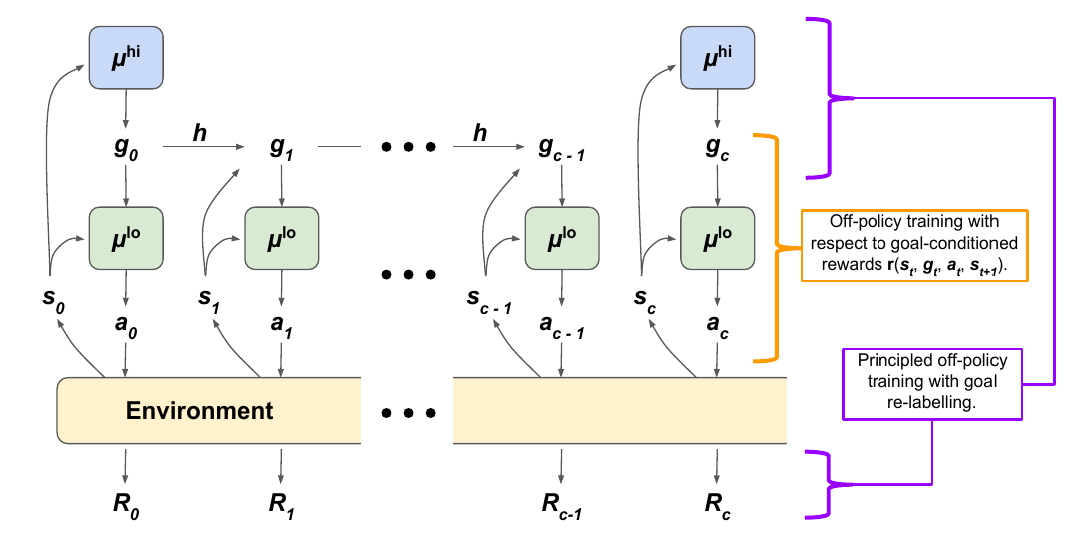
\includegraphics[width=0.8\textwidth]{Images/HIRO.png}
    \caption{HIRO architecture.}
    \label{fig:HIRO}
\end{figure}

